%!TEX root=../slr.tex
\section{Background}
\label{sec:background}

\subsection{Differential Optical Absorption Spectroscopy}
\label{ssub:differential_optical_absorption_spectroscopy}
Absorption Spectroscopy is the term used to identify all techniques that
use radiation absorption by matter to assess and quantify elements or
molecules in a given spectroscopic sample. It had, and still has, a very
important role in the study of the Earth's atmosphere~\cite{Platt2007}.

It is, as many other spectroscopic techniques, based on Lambert-Beer's
law, which states that 'in a medium of uniform transparency the light
remaining in a collimated beam is an exponential function of the length
of the path in the medium', as described originally by Pierre Bouguer in
1729, and can be written~\cite{Platt2007}:
\begin{equation}
    \centering
    I(\lambda) = I_0(\lambda) \cdot \exp[-L \cdot \sigma(\lambda) \cdot c]
    \label{eq:lambert_beer}   
\end{equation}

In Equation~\ref{eq:lambert_beer}, $I$ is the light intensity as measured by the
spectrometer, $I_0$ the original light intensity at the source, $L$ is
the optical path in which the sample is exposed to the light, $\sigma$
is the optical cross section of the sampled element or molecule and $c$
is the sample's concentration. $\lambda$ is the radiation's wavelength.

Lambert--Beer's equation, while valid in a laboratory setting, is
generally not enough to determine gaseous concentrations in an open
atmosphere experiment. $I_0$ determination would require require any
absorbant from the medium, which is impossible. Besides, in this medium,
there are many factors that influence measurements: Rayleigh's
scattering, Mie's scattering, thermal variations, turbulence and
instrumental transmissivities. All these play an important part in
altering atmospheric light~\cite{Platt2007, Merlaud2013}.

Differential Optical Absorption Spectroscopy (DOAS) overcomes these
difficulties by capitalising on cross section's differences between
interfering phenomena (normally broad spectral features) and certain
trace gases (usually narrow spectral structure).  The mathematical
formulations behind the technique are well beyond the scope of this
article, but suffice it to say that the broad structures are removed
through subtraction of a fitted low order polynomial, and a fitting
algorithm (such as Levenberg-Marquardt) is used to retrieve
concentrations. Detailed presentations of these procedures are presented
in~\cite{Platt2007} and~\cite{Merlaud2013}.

In~\cite{Platt2007}, the authors split the DOAS method into two
fundamental families: passive and active. The passive family is
characterised by being designed to capture and analyse natural light,
whether from the Sun, the Moon or any other celestial body. This kind of
measurement has the advantage of being simple to assemble, but natural
light usage implies an additional technical effort for the retrieval of
atmospheric concentrations. Active DOAS applications, on the other hand,
use artificial light sources to make their measurements. This has been
used extensively in the identification of several atmospheric
components. Its concentration extraction procedure is simpler, at the
expense of a more complex assembly.

DOAS has had a number of applications throughout the years. The
technique was first applied in the 1970s. At that time, Perner used an
active setup with a laser light source to identify the OH radical in the
atmosphere~\cite{Perner1976}. More recently, researchers around the
world have been employing broadband sources (such as Xenon lamps) to
measure trace gases like Ozone, Nitrogen Dioxide or Sulphur Dioxide.
Almost simultaneously, passive systems have been used to study
stratospheric chemistry and radiative transport in
clouds~\cite{Platt2007}.

\subsection{Multi-Axis DOAS}%
\label{sub:multi_axis_doas}

Multi-Axis DOAS (MAX-DOAS) is one of the more recent applications of the
DOAS technique. It represents a significant progress regarding zenith
scattered sunlight measurements, a well established atmospheric analysis
technique. It performs a series of passive DOAS measurements in several
telescope elevations (typically 4 to 10)~\cite{Honninger2004}, either in
sequence or simultaneously, according to the schematic representation in
Figure~\ref{fig:max_doas}. 

\begin{figure}[htpb]
    \centering
    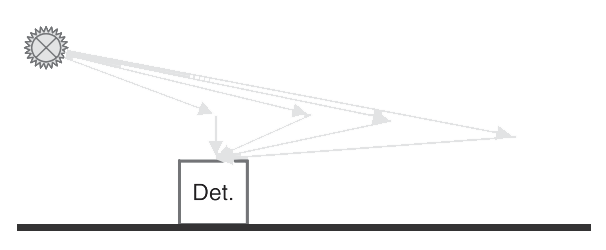
\includegraphics[width=0.8\linewidth]{img/maxdoas.png}
    \caption{MAX-DOAS schematic representation~\cite{Platt2007}.}
    \label{fig:max_doas}
\end{figure}

MAX-DOAS stems from another set of techniques called \emph{off-axis},
which in this case means that the telescope is pointed at another angle
than the zenith. Off-axis DOAS was first employed in 1993 when Sanders
et al.~\cite{Sanders1993} used it to assess OClO in Antarctica. During this
experiment, the team concluded that the off-axis geometry greatly
improves sensitivity for tropospheric species, but does not change the
system's ability to quantify stratospheric absorbers.

By evaluating several directions, the technique allows researchers to
measure not only stratospheric contributors, as zenith sky assemblies,
but also to detect absorbers at ground level, as an active DOAS
instrument would.

We mention MAX-DOAS in this paper because one could argue that these
systems would be able to be adapted to perform tomographic measurements,
if more than one system would analyse the same region from more the same
number of observation angles. MAX-DOAS tomography is a special case, and
would probably deserve to be investigated fully. However, since this was
not the object of our study, we chose not to specifically target this
method in our search.

\subsection{Imaging DOAS}%
\label{sub:imaging_doas}

Imaging DOAS combines spectral and spatial information by combining an
imaging spectrometer with a scanning system. The resulting data clearly
resembles that of a hyperspectrum, as Figure~\ref{fig:idoas_results}
illustrates.

\begin{figure}[htpb]
    \centering
    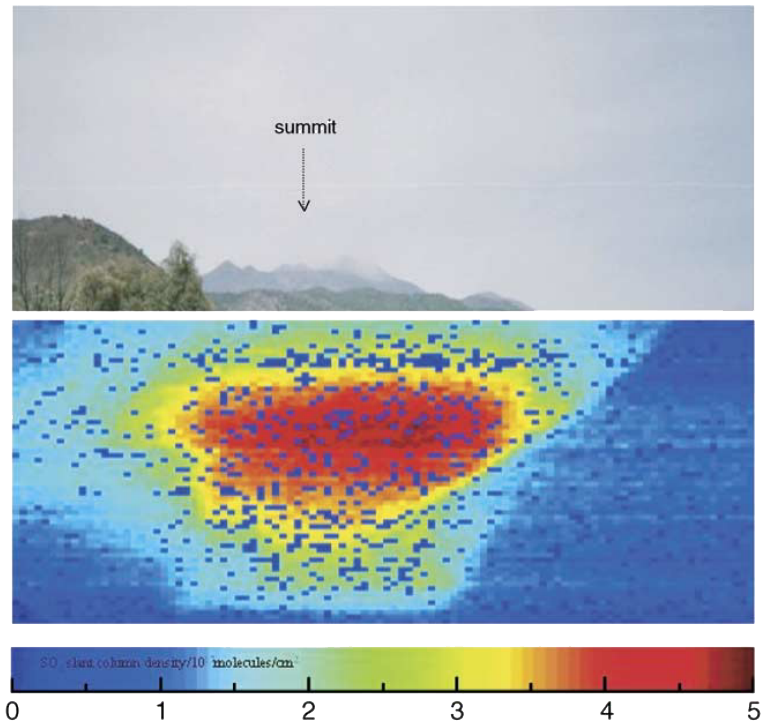
\includegraphics[width=0.5\linewidth]{img/idoas_results.png}
    \caption{IDOAS results over mount Etna, in Italy. The colour coded
    map under the digital photograph represents the SO$_2$
concentration~\cite{Bobrowski2006}.}
\label{fig:idoas_results}
\end{figure}

The method, developed by Bobrowsky et al.~\cite{Bobrowski2006}, employs a 2D
CCD detector. One dimension measures spectral information, while the
other contains spatial information for one direction. The other spatial
direction is obtained by scanning the field of view with the pushbroom
method. A schematic representation is presented in the same article, and
is here reproduced in Figure~\ref{fig:idoas_schematic}.

\begin{figure}[htpb]
    \centering
    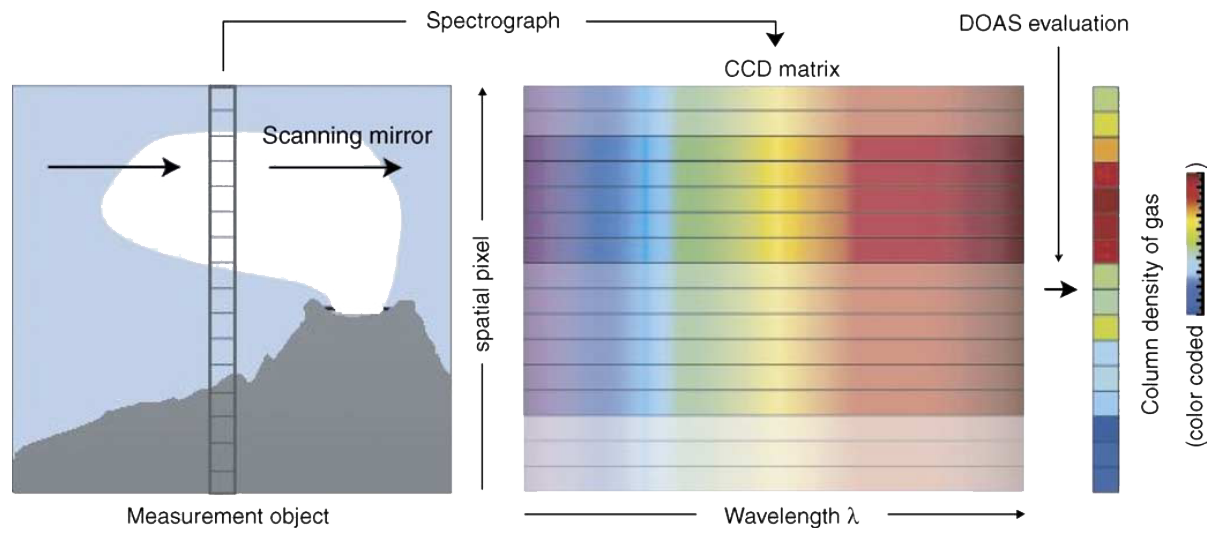
\includegraphics[width=0.8\linewidth]{img/idoas_schematic.png}
    \caption{IDOAS capture functioning schematic ~\cite{Bobrowski2006}.}
    \label{fig:idoas_schematic}
\end{figure}

DOAS is used to yield slant column density values for the absorbers for
each pixel. The values are colour coded and produce an image describing
the gas distribution.

This technique is included in this paper because it exists in order to
produce a two-dimensional image from spectral information. This image,
however, does not come from a tomographic reconstruction procedure, nor
is spatial information recovered from projections, but instead comes
directly from the acquisition method. Hence, we did not include articles
on this method in this study.
% END DOAS

\subsection{Tomography}
\label{sub:tomography}
Tomography refers to the set of techniques that aim to produce a cross
sectioning image from data collected by exposing a given target body to
some kind of penetrating or reflecting wave from many different
directions~\cite{Herman2009, Kak2001a}.

The initial theories that gave rise to tomography were laid out by
Johannes Radon in 1917, with a mathematical operation that  would later
be known as the Radon transform. This process maps a function f, defined
in the plane, to the function Rf, comprised of the values of the line
integrals of f, taken in $\theta$ directions. In practice, this
formulation allows the reconstruction of an image by its projections,
which are nothing more than line integrals~\cite{Feeman2010}.

Tomographic image reconstruction can be achieved by running one of
several algorithms through a computer program. The presentation of these
algorithms is completely beyond the scope of this article, but a good
starting point for learning about these operations is \emph{The
Mathematics of Medical Imaging}, by Timothy Feeman~\cite{Feeman2010}. It
is in the scope of this article, however, to make a small introduction
to a particular set of reconstruction methods. The reason for this being
the prevalence of these methods in the field of DOAS tomography, which
is the main subject of this study. These techniques are thus:
\begin{description}
    \item[Algebric Reconstruction Techniques (ART)] Proposed in 1970 by
        Gordon and Herman~\cite{Herman1973}, these techniques are based
        on successive approximations between the actual projection data
        and the sum of the reconstruction elements which represent
        it~\cite{Gordon1974}. The process is conducted line by line,
        until a satisfactory convergence condition is met.

    \item[Simultaneous ART] Simultaneous ART is very similar to the ART
        algorithm. The difference being that the iterative changes occur
        for all lines at the same time, instead of in only one.

    \item[Simultaneous Iterative Reconstruction Techniques (SIRT)] The
        main difference between SIRT and SART is that in the former,
        cell changes are not reflected immediately after one
        calculation. Updates occur at the end of each iteration. At this
        point, the change for each cell is the average correction
        calculated for it taking all equations into
        account~\cite{Kak2001}.
\end{description}

During the second half of the twentieth century, tomographic processes
have had a revolutionary influence in many fields of study, but
especially in medicine (see Figure~\ref{fig:ct_scan}). Computational
tomography scanners allow doctors to see their patients interior in a
highly detailed and extremely safe fashion. At first, tomographic
imaging was performed only with X-Rays.  Their attenuation throughout
the patient's body being used as a projection. Nowadays, there are much
more methods of image retrieval, such as radioisotopes, ultrasound or
particle anihilation~\cite{Kak2001a, Feeman2010, Herman2009}.

\begin{figure}[htb]
    \centering
    % \includegraphics[width=0.8\linewidth]{ct_scan.png}
    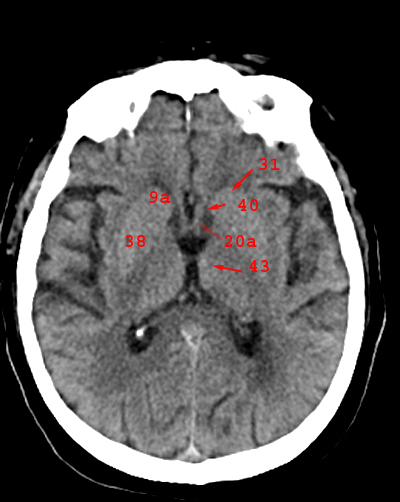
\includegraphics[width=0.6\textwidth]{img/CT07.jpg}    
    \caption{Tomographic image, axial view of the human
        brain~\cite{Glowniak}. Note how a trained clinician can identify
        several structures (7 red notes) with just one slice of a
        computerised tomography image. Before tomographic techniques
        were invented, it was impossible to retrieve this this kind of
        detail without dissecting the patient.}
    \label{fig:ct_scan}
\end{figure}

Although it was the field of medicine was more influenced by tomographic
procedures than any other, the applications of these methods are not
restricted to it. One can find numerous industrial and research
applications~\cite{Wang2015, Haisch2012, Byer1979}. One of which is the
application to atmospheric research, namely in conjunction with DOAS. In
recent years, scientists have been working on tomographic methods for
measuring atmospheric trace gas concentration values. The field is
interesting because it allows for 2D or even 3D mapping of a given
region, with respect to those trace gases. This article aims to make an
assessment of the status of this tomographic application, by analysing
current literature on the subject. 
%END TOMOGRAPHY



\subsection{Mapping Study}
\label{sub:mapping_study}

A Systematic Mapping Study (MS) is a type of secondary study designed to
determine the general features of the research landscape in the subject
they are addressing~\cite{Kitchenham2007, Petersen2008}.

An MS is driven by broad (and often multiple) research questions and
applies an also broad data extraction protocol. This is in line with the
fact that this kind of study aims to summarise its findings, answering
the research questions, and in-depth analysis is not required. It is
common for an MS to be a precursor to a Systematic Literature Review
(SLR), which is a much deeper kind of systematic study. Guidelines for
performing studies of both kinds can be found in a report made by
Kitchenham and Charters in 2007~\cite{Kitchenham2007}. In this document,
the authors establish the 3 stages which all MS and SLR generally have:

\begin{description}
    \item[Planning] This stage includes all preliminary considerations
        regading the MS or SLR in the making. All protocols, from search
        to evaluation, through data extraction, are devised;
    \item[Conduction] During this staged, researchers apply what they
        have planned in the previous phase. Protocols are
        \emph{actually} run, and data is synthesised;
    \item[Reporting] In this phase, the team has to define their
        dissemination strategy, and implement it. It is in this stage
        that a final report is written and evaluated.
\end{description}

Although it is logical (and fundamentally correct) to assume that these
steps are sequential, this may not be, and usually is not, accurate.
Many of these stages and their intermediate steps require iteration. For
instance, some inclusion or exclusion criteria may only be found
necessary once the search protocol is implemented.

% End Mapping Study
%\subsection{Methods}
%\label{sub:methods}

%Given our goals and the particular methodology that we have chosen to
%adopt with this study, it is important to provide a small introduction
%to how we have planned to proceed and what we will be evaluating.

%\subsection{Research Questions}
%\label{sub:research_questions}

%As stated in Kitchenham's 2007 report~\cite{Kitchenham2007}, Research
%Questions (RQ) are what drives every MS. There are several types of
%research question. They can be focused on costs, advantages or
%assessment of a given technology or procedure. In our case, we are more
%interested in this latter type. The literature on SLR and MS recommend
%establishing RQs by considering them through some standard viewpoints, a
%guideline that is refered to as a PICOC analysis:

%\begin{description}
%    \item[Population] the ones affected by the study or the technology
%        that is being assessed;
%    \item[Intervention] the specific methodology or tool which will be
%        applied to the subject of interest, with the MS goals in mind;
%    \item[Comparison] a benchmark with which to compare obtained
%        results;
%    \item[Outcomes] the expected results of the MS or SLR study in
%        question.
%\end{description}

%A more profound analysis of how our RQ are defined can be found in
%Section~\ref{sec:methods}, but since our goal is to map research
%literature on the subject of DOAS tomography, our main research question
%is \textbf{\emph{What is the current status of the technology used in
%tomographic DOAS?}}.
%% End of Research Questions

%\subsection{Data Extraction Strategy}
%\label{sub:data_extraction_strategy}

%After having defined the RQ, it is important to plan how the study will
%try to answer those questions. This is to say a \emph{data extraction
%strategy}. It includes the choice of libraries, the definition of a
%search string, exclusion and inclusion filters,  and the scoring method
%for each article. It also includes the description of how the data is to
%be assessed within each paper. 

%Section~\ref{sec:methods} includes a complete description of how this is
%approached, while a summarised presentation of how we have approached
%this is illustrated in Table~\ref{tab:data_extraction_summary}.

%\begin{table}[htb]
%    \centering
%    \caption{Data extraction: a small summary.}
%    \label{tab:data_extraction_summary}
%    \begin{small}
%        \begin{tabular}{@{}ll@{}}
%        \toprule
%        \multirow{5}{*}{\textbf{Libraries Searched}} & Google Scholar\\
%                                                    & IEEE\\
%                                                    & Web of Knowledge\\
%                                                    & Science Direct\\
%                                                    & American Geophysical Union\\ \midrule
%        \textbf{Search String}                      & DOAS atmospher* tomography                \\ \midrule
%        \multirow{5}{*}{\textbf{Exclusion Filters}} & Duplicate in Scholar                      \\
%                                                    & Non English articles are not accepted     \\
%                                                    & Satellite data papers are not accepted    \\
%                                                    & Volcanology papers are not accepted       \\
%                                                    & CNKI published articles are not accepted  \\ \midrule
%        \multirow{2}{*}{\textbf{Inclusion Filters}} & Must be full articles                     \\
%                                                    & Must be about Tomographic DOAS            \\ \midrule
%        \textbf{Papers found}                       & 732                                       \\ \midrule
%        \textbf{Papers discarded}                   & 724                                       \\ \midrule
%        \multirow{2}{*}{\textbf{Screening methods}} & 1. Abstract analysis to produce shortlist \\
%                                                    & 2. Full read of shortlisted articles      \\ \midrule
%        \textbf{Analysed papers}                    & 8                                         \\ \bottomrule
%        \end{tabular}    
%    \end{small}
%\end{table}
%%End of Libraries
%%End of Methods

%\subsection{Results}
%\label{sub:results}

%As can be seen in Table~\ref{tab:data_extraction_summary}, our search
%returned around 730 results, of which a small fraction (8) managed to
%pass all exclusion and inclusion filters we had defined. With reference
%to the structure of the retrieved results, it is important to note that
%most of the results (80\%) came from Google Scholar.

%As to the analysis, we have found that instrument descriptions were
%found in 6/8 articles; algorithm descriptions in 5/8 articles, and
%software mentions in 3/8 articles. We have also found that there were
%5/8 empirical papers (associated to an experiment) while the
%remaining 3/8 were theoretical papers. Following our scoring method
%(defined in Table~\ref{tab:quality_assessment_criteria}), our 8 articles
%had achieved an average score of 0,48, with a median of 0,6. Although
%the sample is very small, this disparity between average and median
%hints at the existence of outliers or some kind of clustering.

%As to the setup information that we have set out to obtain, we were able
%to extract several instrument configurations, algorithms and used
%software, which are presented and discussed in
%Section~\ref{sec:conduction}. 
%%End of Results

%\subsection{Conclusions}
%\label{sub:conclusions}

%DOAS tomography has many possible applications and many possible
%interested parties. However, literature on the subject, especially in
%what refers to urban, rural or industrial scenarios is limited. The
%technology used for the different systems surveyed in this study is
%mostly the same active DOAS setup, granted some peculiarities of each
%system. The method is also very research-focused, although some
%researchers seem to be near a commercial/industrial application.

%%End of Conclusions
